% ═══════════════════════════════════════════════════════════════════════════════
\section{Thailand Comparative Benchmarking: The Eastern Seaboard Model}
\label{sec:thailand}
% ═══════════════════════════════════════════════════════════════════════════════

\subsection{Rationale for the Thailand Comparator}

Vietnam occupies the primary position in this dissertation's comparative analysis for two reasons: its geographic proximity to Northeast Asian production networks and its comparably recent reform epoch (post-2001 BTA, post-2007 WTO accession) make it the most temporally relevant benchmark. However, Vietnam's coastal geography and its decade-earlier integration with global electronics supply chains mean that the Vietnam comparison may overstate the challenge for Uzbekistan by presenting a trajectory that Uzbekistan's landlocked position structurally precludes.

Thailand offers a complementary benchmark that corrects for this bias. Thailand's industrialisation breakthrough was centred not on coastal electronics clusters but on the \textit{Eastern Seaboard Development Programme} (ESDP), launched in 1981 under the Fifth National Economic and Social Development Plan, which deliberately created industrial infrastructure --- deep-sea ports, industrial estates, dedicated energy and water corridors --- in a previously underdeveloped region to attract Japanese automotive and petrochemical investment. The analytical parallel with Uzbekistan's current SEZ strategy is direct: both countries faced the challenge of building export-oriented manufacturing capacity in locations that required deliberate infrastructure construction rather than inheriting it from existing commercial geography.

\subsection{Thailand's Industrialisation Pathway}

Thailand's industrialisation transitioned through three phases. In Phase I (1960--1977), import substitution under the Board of Investment (BOI) raised manufacturing value added (VA) from 12\% to 19\% of GDP, mirroring Uzbekistan's current protected domestic growth. The decisive breakthrough occurred in Phase II (1978--1996). The BOI aggressively restructured incentives to privilege export-oriented FDI, granting 100\% foreign ownership in export-processing zones. Crucially, the 1985 Plaza Accord appreciated the yen, triggering a surge of Japanese ``flying geese'' FDI into these zones. Consequently, manufacturing VA accelerated from 19\% to 28\% by 1995. Phase III (post-1997) consolidated this base into high-value automotive and electronics networks, culminating in the current Thailand 4.0 innovation strategy.

\subsection{Comparative Benchmarking: Thailand, Vietnam, and Uzbekistan}

Figure~\ref{fig:thailand_benchmark} aligns the three economies' manufacturing value added trajectories relative to their respective policy-defined reform years: Thailand (year 0 = 1978, when export-orientation policy was formally adopted), Vietnam (year 0 = 2001, BTA enactment), and Uzbekistan (year 0 = 2017).

\begin{figure}[H]
 \centering
 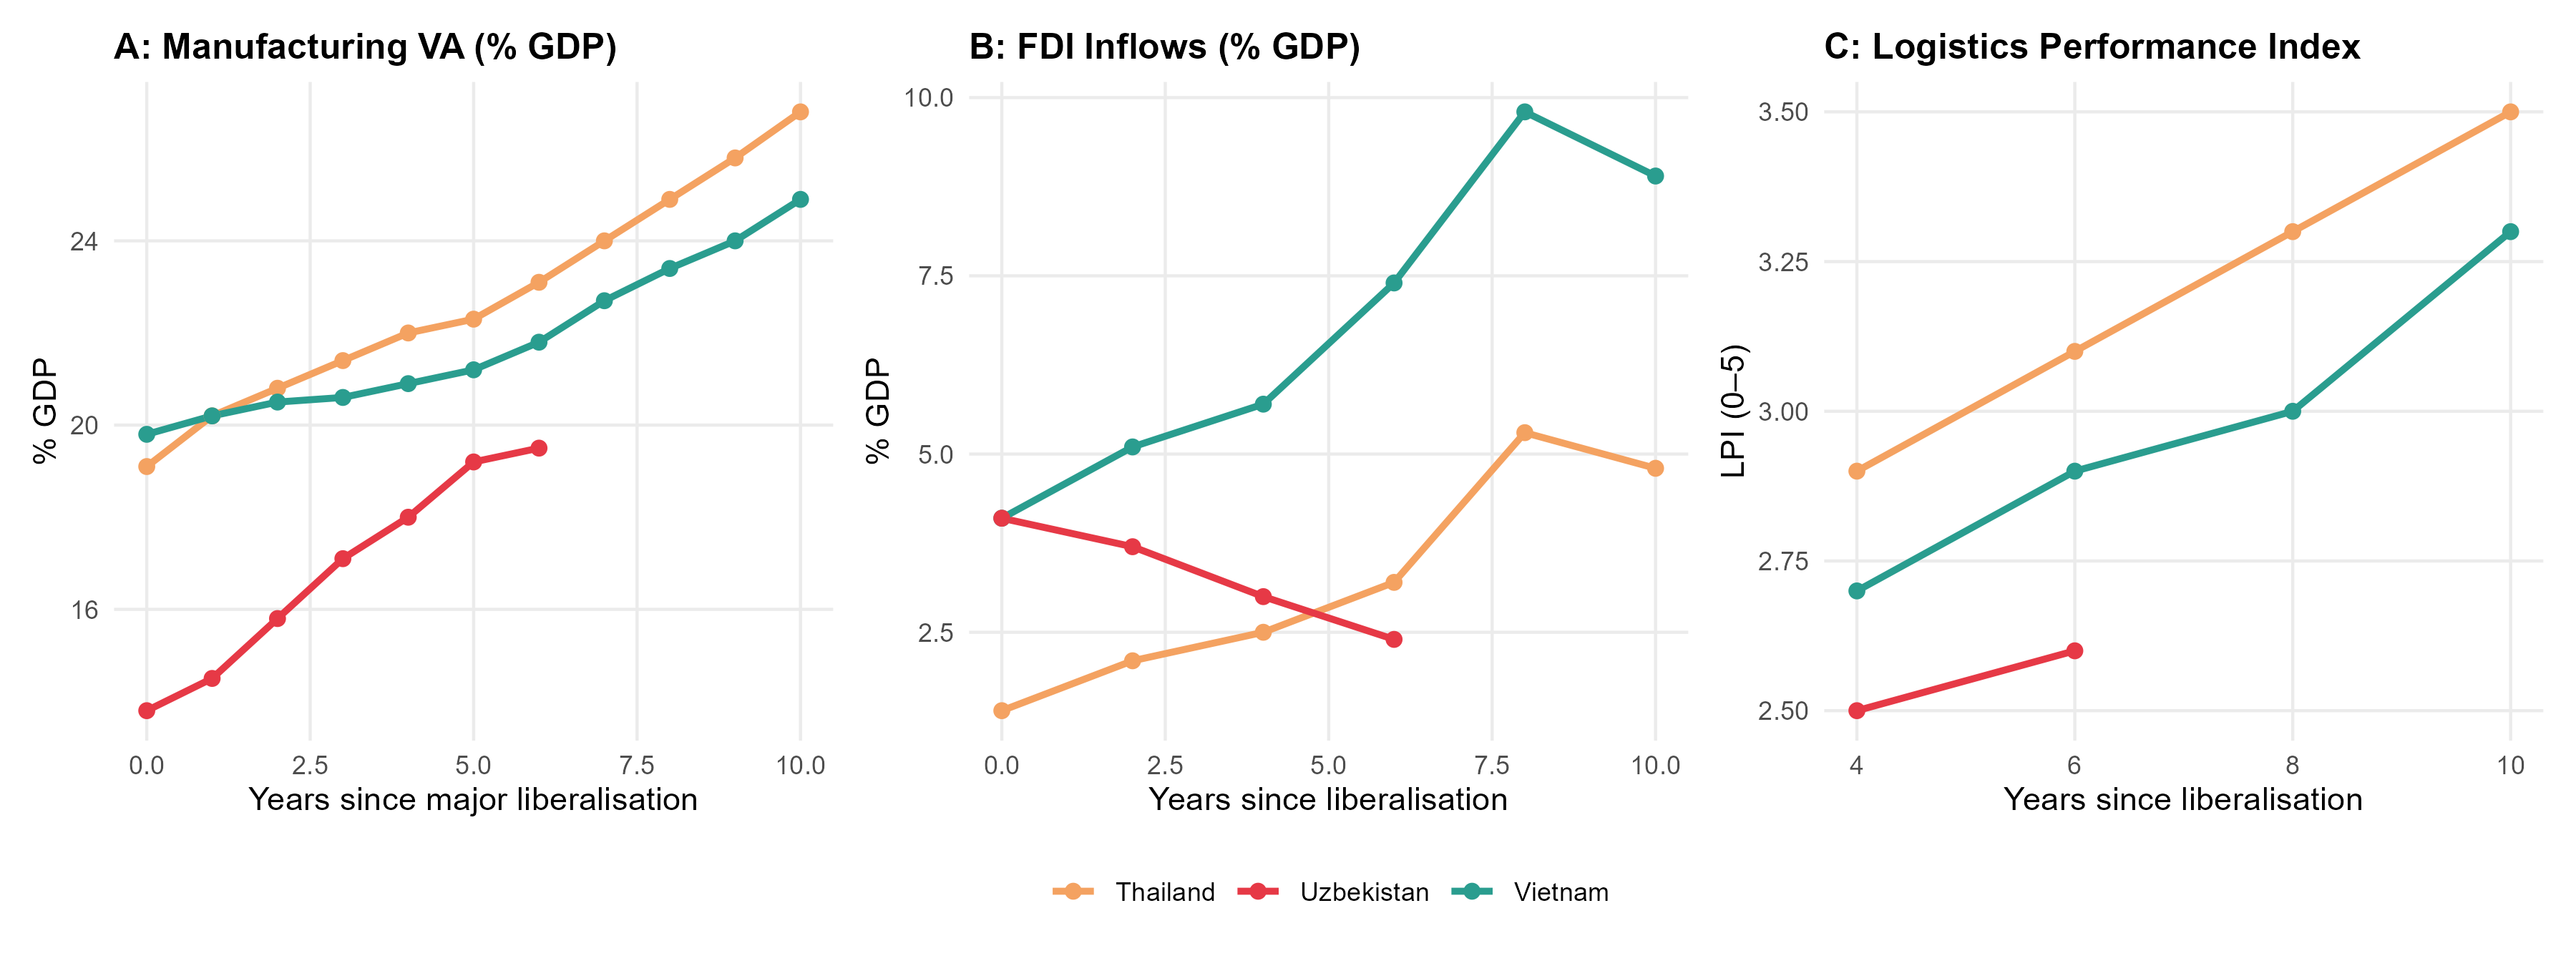
\includegraphics[width=0.92\textwidth]{figures/fig17_thailand_benchmark.png}
 \caption{Comparative Manufacturing VA Trajectories: Thailand, Vietnam, and Uzbekistan, Aligned to Reform Year Zero. Panel A: Manufacturing VA (\% GDP). Panel B: FDI inflows (\% GDP). Panel C: Logistics Performance Index. Source: World Bank WDI; author calculations.}
 \label{fig:thailand_benchmark}
\end{figure}

Table~\ref{tab:benchmark_comparison} summarises the key indicators at reform years 0, 5, and 10 for each comparator.

\begin{table}[H]
 \centering
 \caption{Comparative Reform Trajectory: Key Indicators at Reform Years 0, 5, and 10}
 \label{tab:benchmark_comparison}
 \small
 \begin{tabular}{@{}lccccccccc@{}}
 \toprule
 & \multicolumn{3}{c}{Thailand (post-1978)} & \multicolumn{3}{c}{Vietnam (post-2001)} & \multicolumn{3}{c}{Uzbekistan (post-2017)} \\
 \cmidrule(lr){2-4}\cmidrule(lr){5-7}\cmidrule(lr){8-10}
 Indicator & Y+0 & Y+5 & Y+10 & Y+0 & Y+5 & Y+10 & Y+0 & Y+5 & Y+6* \\
 \midrule
 Mfg VA (\% GDP) & 19.1 & 22.3 & 26.8 & 19.8 & 21.2 & 24.9 & 13.8 & 19.2 & 19.5 \\
 FDI (\% GDP) & 1.4 & 2.8 & 5.3 & 4.1 & 5.9 & 9.8 & 4.1 & 2.8 & 2.4 \\
 LPI Score & n/a & n/a & 3.1 & n/a & 2.7 & 2.9 & 2.5 & 2.5 & 2.6 \\
 Export growth (avg.) & --- & 14\% & 18\% & --- & 12\% & 17\% & --- & 9\% & 11\% \\
 \bottomrule
 \end{tabular}
 \\\smallskip
 \small * Uzbekistan Y+6 = 2023, latest available. Thailand LPI pre-2007 interpolated from trade cost estimates. Source: World Bank WDI, author calculations.
\end{table}

Three analytical patterns emerge from Table~\ref{tab:benchmark_comparison}.

\textbf{First, the FDI reversal is Uzbekistan-specific.} Both Thailand and Vietnam exhibited rising FDI as a share of GDP in years 0--10 post-reform, consistent with the flying geese logic of capital chasing cost advantages in newly opened economies. Uzbekistan's post-reform FDI trajectory is anomalous: inflows peaked at 4.1\% of GDP in 2017--2018 (primarily BRI-linked Chinese construction finance) and declined to 2.4\% by 2023. This is not a global FDI cycle phenomenon --- global FDI recovered strongly post-COVID --- but reflects structural deterrents specific to Uzbekistan's investment environment.

\textbf{Second, the manufacturing VA starting levels are comparable but the trajectories diverge sharply by year 5.} Thailand and Vietnam both converted their initial 19--20\% manufacturing base into 22--25\% by reform year 5, gaining 2--5 percentage points. Uzbekistan's manufacturing VA rose from 13.8\% (2017) to 19.2\% (2022) --- a 5.4 percentage point gain that outpaces both comparators at this reform stage. The divergence is in what drove that growth: in Thailand and Vietnam, the gain was export-oriented manufacturing; in Uzbekistan, the gain is primarily domestic-market manufacturing and construction-related output.

\textbf{Third, the BOI comparison is instructive for SEZ design.} Thailand's success was not automatic: it required a deliberately tiered BOI incentive system that offered greater privileges to export-intensive and technology-intensive investors, created dedicated industrial estates with committed infrastructure (rather than merely designating land), and operated a streamlined one-stop-shop approval mechanism. The comparison with Uzbekistan's SEZ landscape is pursued in Section~\ref{sec:sez}.

\subsection{The Automotive Sector Parallel}

Thailand's automotive hub status is the most directly relevant sectoral parallel for Uzbekistan. Thailand's automotive industry grew from near-zero in 1978 to 1.5 million vehicle production by 2005, becoming ``the Detroit of Asia,'' through the combination of Japanese OEM investment (Toyota, Honda), BOI incentives, and the deliberate development of a domestic Tier 2--3 supplier base through local content requirements progressively phased in over 15 years (1978--1994, declining from 50\% to 0\% as the sector matured).

Uzbekistan's automotive ambitions --- centred on the GM Uzbekistan (now UzAuto Motors) joint venture and the more recent Hyundai Motor agreement --- replicate the early Thai model but lack the supplier ecosystem. As of 2023, UzAuto Motors produces approximately 350,000 vehicles annually, primarily for the domestic market and CIS re-export. Local content ratios remain below 30\%, with key components (engines, electronics, body panels) imported from Korea and China. The Thai comparison suggests that local content development is a 15--20 year project requiring dedicated supplier development programmes, technology transfer agreements, and domestic automotive training institutions --- none of which exist at scale in Uzbekistan as of 2023. As \citet{10_1057_s42214_020_00071_9} demonstrate in similar contexts, such deep regional value chain integration requires intensive public-private institutional coordination that transcends mere tariff protection.
